%%
%% This is file `sample-sigconf.tex',
%% generated with the docstrip utility.
%%
%% The original source files were:
%%
%% samples.dtx  (with options: `sigconf')
%% 
%% IMPORTANT NOTICE:
%% 
%% For the copyright see the source file.
%% 
%% Any modified versions of this file must be renamed
%% with new filenames distinct from sample-sigconf.tex.
%% 
%% For distribution of the original source see the terms
%% for copying and modification in the file samples.dtx.
%% 
%% This generated file may be distributed as long as the
%% original source files, as listed above, are part of the
%% same distribution. (The sources need not necessarily be
%% in the same archive or directory.)
%%
%% The first command in your LaTeX source must be the \documentclass command.
\documentclass[sigconf]{acmart}
\usepackage{graphicx} 
\usepackage{multirow}
\usepackage{xcolor}
\usepackage[normalem]{ulem}
\useunder{\uline}{\ul}{}
%%
%% \BibTeX command to typeset BibTeX logo in the docs
\AtBeginDocument{%
  \providecommand\BibTeX{{%
    \normalfont B\kern-0.5em{\scshape i\kern-0.25em b}\kern-0.8em\TeX}}}

%% Rights management information.  This information is sent to you
%% when you complete the rights form.  These commands have SAMPLE
%% values in them; it is your responsibility as an author to replace
%% the commands and values with those provided to you when you
%% complete the rights form.
\setcopyright{acmcopyright}
\copyrightyear{2018}
\acmYear{2018}
\acmDOI{10.1145/1122445.1122456}

%% These commands are for a PROCEEDINGS abstract or paper.
\acmConference[Woodstock '18]{Woodstock '18: ACM Symposium on Neural
  Gaze Detection}{June 03--05, 2018}{Woodstock, NY}
\acmBooktitle{Woodstock '18: ACM Symposium on Neural Gaze Detection,
  June 03--05, 2018, Woodstock, NY}
\acmPrice{15.00}
\acmISBN{978-1-4503-XXXX-X/18/06}


%%
%% Submission ID.
%% Use this when submitting an article to a sponsored event. You'll
%% receive a unique submission ID from the organizers
%% of the event, and this ID should be used as the parameter to this command.
%%\acmSubmissionID{123-A56-BU3}

%%
%% The majority of ACM publications use numbered citations and
%% references.  The command \citestyle{authoryear} switches to the
%% "author year" style.
%%
%% If you are preparing content for an event
%% sponsored by ACM SIGGRAPH, you must use the "author year" style of
%% citations and references.
%% Uncommenting
%% the next command will enable that style.
%%\citestyle{acmauthoryear}

%%
%% end of the preamble, start of the body of the document source.
\begin{document}

%%
%% The "title" command has an optional parameter,
%% allowing the author to define a "short title" to be used in page headers.
\title{Efficient and Bias-aware Recommendation with Two-side Relevance for Implicit Feedback}

%%
%% The "author" command and its associated commands are used to define
%% the authors and their affiliations.
%% Of note is the shared affiliation of the first two authors, and the
%% "authornote" and "authornotemark" commands
%% used to denote shared contribution to the research.
\author{Ben Trovato}
\authornote{Both authors contributed equally to this research.}
\email{trovato@corporation.com}
\orcid{1234-5678-9012}
\author{G.K.M. Tobin}
\authornotemark[1]
\email{webmaster@marysville-ohio.com}
\affiliation{%
  \institution{Institute for Clarity in Documentation}
  \streetaddress{P.O. Box 1212}
  \city{Dublin}
  \state{Ohio}
  \postcode{43017-6221}
}

\author{Lars Th{\o}rv{\"a}ld}
\affiliation{%
  \institution{The Th{\o}rv{\"a}ld Group}
  \streetaddress{1 Th{\o}rv{\"a}ld Circle}
  \city{Hekla}
  \country{Iceland}}
\email{larst@affiliation.org}

\author{Valerie B\'eranger}
\affiliation{%
  \institution{Inria Paris-Rocquencourt}
  \city{Rocquencourt}
  \country{France}
}

\author{Aparna Patel}
\affiliation{%
 \institution{Rajiv Gandhi University}
 \streetaddress{Rono-Hills}
 \city{Doimukh}
 \state{Arunachal Pradesh}
 \country{India}}

\author{Huifen Chan}
\affiliation{%
  \institution{Tsinghua University}
  \streetaddress{30 Shuangqing Rd}
  \city{Haidian Qu}
  \state{Beijing Shi}
  \country{China}}

\author{Charles Palmer}
\affiliation{%
  \institution{Palmer Research Laboratories}
  \streetaddress{8600 Datapoint Drive}
  \city{San Antonio}
  \state{Texas}
  \postcode{78229}}
\email{cpalmer@prl.com}

\author{John Smith}
\affiliation{\institution{The Th{\o}rv{\"a}ld Group}}
\email{jsmith@affiliation.org}

\author{Julius P. Kumquat}
\affiliation{\institution{The Kumquat Consortium}}
\email{jpkumquat@consortium.net}

%%
%% By default, the full list of authors will be used in the page
%% headers. Often, this list is too long, and will overlap
%% other information printed in the page headers. This command allows
%% the author to define a more concise list
%% of authors' names for this purpose.
\renewcommand{\shortauthors}{Trovato and Tobin, et al.}

%%
%% The abstract is a short summary of the work to be presented in the
%% article.
\begin{abstract}
	Today's wide-spread recommendation is usually constructed based on implicit data such as click for easy collection but whether the no clicked data is negative feedback or unobserved positive feedback confuses the model construction. As a response, Relevance Matrix Factorization (Rel-MF) is recently proposed to tackle this problem as well as the missing-not-at-random (MNAR) problem ignored by previous studies. However, Rel-MF meets three problems$\colon$ limited assumption (LA), negative square loss (NSL) and indiscriminate no click data (INCD). In this paper, we first get rid of Rel-MF's limited assumption and establish a more general theory by incorporating a defined transformation function which captures the relevance level to our two-side relevance ideal loss, containing Rel-MF's theory. To resolve the INCD problem and NSL problem, we introduce an adjusting variable and perform normalization, respectively, which is called Naive Solution with Normalization for Rel-MF (NRel-MF). But we then analytically discover that the clipped function proposed by Rel-MF meets the high variance problem. To overcome it, we design a power clipped function and further propose Improved Solution with Power Function for Rel-MF (PRel-MF). Besides, we also explore propensity score estimation from user and hybrid perspectives in contrast to Rel-MF's sole item perspective. Finally, we also consider and address the computational problem caused by the Rel-MF's non-sampling strategy. Empirical results verify the effectiveness of our solutions from both performance even in rare items and loss decrease. In broader perspective experiment, decent performance is seen in item perspective with fewer recommended items while in user perspective with more recommended items and hybrid perspective outperforms them in more situations.  
\end{abstract}

%%
%% The code below is generated by the tool at http://dl.acm.org/ccs.cfm.
%% Please copy and paste the code instead of the example below.
%%
\begin{CCSXML}
<ccs2012>
 <concept>
  <concept_id>10010520.10010553.10010562</concept_id>
  <concept_desc>Computer systems organization~Embedded systems</concept_desc>
  <concept_significance>500</concept_significance>
 </concept>
 <concept>
  <concept_id>10010520.10010575.10010755</concept_id>
  <concept_desc>Computer systems organization~Redundancy</concept_desc>
  <concept_significance>300</concept_significance>
 </concept>
 <concept>
  <concept_id>10010520.10010553.10010554</concept_id>
  <concept_desc>Computer systems organization~Robotics</concept_desc>
  <concept_significance>100</concept_significance>
 </concept>
 <concept>
  <concept_id>10003033.10003083.10003095</concept_id>
  <concept_desc>Networks~Network reliability</concept_desc>
  <concept_significance>100</concept_significance>
 </concept>
</ccs2012>
\end{CCSXML}

\ccsdesc[500]{Computer systems organization~Embedded systems}
\ccsdesc[300]{Computer systems organization~Redundancy}
\ccsdesc{Computer systems organization~Robotics}
\ccsdesc[100]{Networks~Network reliability}

%%
%% Keywords. The author(s) should pick words that accurately describe
%% the work being presented. Separate the keywords with commas.
\keywords{datasets, neural networks, gaze detection, text tagging}

%% A "teaser" image appears between the author and affiliation
%% information and the body of the document, and typically spans the
%% page.
%\begin{teaserfigure}
%  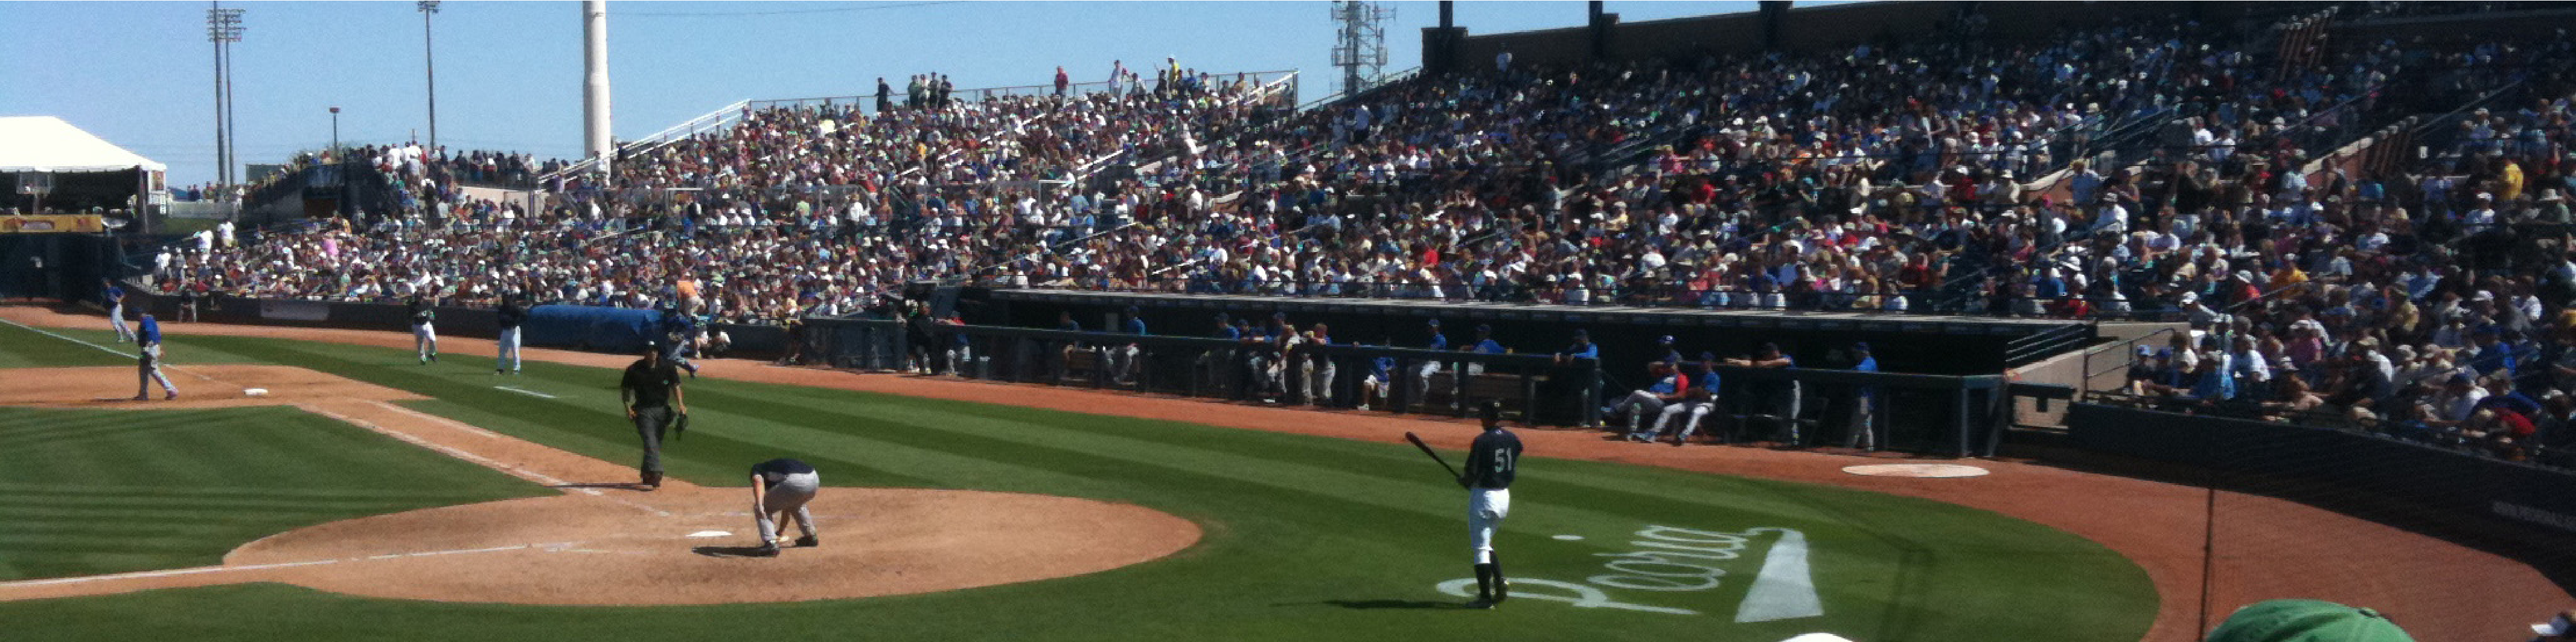
\includegraphics[width=\textwidth]{sampleteaser}
%  \caption{Seattle Mariners at Spring Training, 2010.}
%  \Description{Enjoying the baseball game from the third-base
%  seats. Ichiro Suzuki preparing to bat.}
%  \label{fig:teaser}
%\end{teaserfigure}

%%
%% This command processes the author and affiliation and title
%% information and builds the first part of the formatted document.
\maketitle

\section{Introduction}
	With the exploration of information, the construction of some intelligent systems like recommendation systems is becoming more and more common~\cite{ricci2011introduction}. The wide-spread recommendation~\cite{xue2017deep, liu2010personalized} is now helping us to make choice more conveniently in daily life. Actually, recommender systems facilitate user's purchasing behavior and give them better shopping experience~\cite{schafer1999recommender}. The mechanism of recommendation is to model and predict the users' preference towards items.

A few decades have seen the growth of recommendation methods and collaborative filtering (CF)~\cite{Goldberg-CF-92} is a widely applied technique. Probabilistic matrix factorization~\cite{NIPS2007-PMF} is a typical model in CF, which utilizes explicit feedback data. Apart from explicit feedback data, there is also another type of data about implicit feedback. Explicit feedback with rating data can indicate us about the users' preferences. But it is difficult for us to collect it for providing rating feedback may be a troublesome requirement for many users~\cite{jannach2018recommending}. On the contrary, implicit feedback data, such as click or scan, is much easier for us to obtain and many recommender systems are actually based on it~\cite{liu2010personalized, chen2020efficient}. Indeed, for information retrieval fields~\cite{joachims2016counterfactual, joachims2017unbiased, wang2018position} including recommendation, modeling the relevance of users towards items accurately based on implicit feedback is a significant task because it determines whether the users can be recommended with their truly preferred items. However, there existing no click data confusing us for it is impossible for us to discriminate whether it is negative feedback or positive feedback but unobserved yet, leading to positive unlabeled problem~\cite{elkan2008learning, bekker2019beyond}. There is also some work tackling this problem via negative sampling~\cite{xu2016tag}, but actually non-negative sampling strategy can reach more optimal and stable convergence for its gradient is calculated by the whole data (including no click data)~\cite{chen2019efficient, hu2008collaborative}.

To tackle the positive unlabeled problem, Weighted Matrix Factorization (WMF)~\cite{hu2008collaborative} is proposed via assigning less weight to the loss of no click data. But they treat the no click data as the same while there is supposed to be discrimination within no click data (i.e. INCD problem). Based on the fact that more times recommended items with no click are less relevant, Exposure Matrix Factorization (ExpoMF) is then proposed~\cite{liang2016modeling}. Incorporating exposure to items into Matrix Factorization (MF)~\cite{NIPS2007-PMF}, ExpoMF assigns more weight to the loss of data with higher exposure. Successfully addressing the positive unlabeled problem, ExpoMF fails to tackle the missing-not-at-random (MNAR)~\cite{schnabel2016recommendations, yang2018unbiased} problem because weighting more on the loss of data for popular items (with high exposure) is unfair for rare items and results in poor modeling performance for them. 

To address these two bias problems (i.e. the positive unlabeled problem and MNAR problem), Relevance Matrix Factorization (Rel-MF)~\cite{saito2020unbiased} is further proposed, weighting the loss with relevance instead of click probability. More specifically, an ideal loss function is first defined with optimization of maximizing the relevance. Then they tackle the positive unlabeled problem and MNAR problem based on the causal inference predicting technique~\cite{rubin1974estimating, rosenbaum1983central, imbens2015causal}. Finally, to reduce the variance they further propose a clipped estimator and project the propensity score~\cite{rosenbaum1983central} via item popularity. However, they ignore the INCD problem WMF meets and also does not discriminate between the no click data for the weight of their final proposed clipped estimator would be the same within no click data (i.e. INCD Problem in Section~\ref{sec:rmf}). Besides, their solution also sees negative value in square loss, which is unreasonable for the target of square loss should be 0 and its value is often greater than 0 (i.e. NSL Problem in Section~\ref{sec:rmf}). More importantly, the proof of their defined ideal loss is not general (i.e. LA Problem in Section~\ref{sec:rmf}), resulting in the limitation of their established theory. These problems Rel-MF meets facilitate us to design a stronger model. In this work, we first remake the assumption and establish a more general theory by introducing the transformation function to capture the relationship of relevance level with the click probability and exposure probability in our two-side relevance ideal loss, aiming to address LA problem. After including their clipped estimator to our established theory, we then propose a naive solution with normalization for Rel-MF (NRel-MF), introducing an adjusting variable to tackle INCD problem and we address NSL problem naively via normalization. However, on the analysis of normalized clipped function, we discover that the clipped function developed based on this paper~\cite{saito2020unbiased} suffers from a high variance problem, facilitating us to design a new clipped function based on power function (PRel-MF). Experimental results also confirm the effectiveness of our proposed solutions from both performance and loss decrease. Besides, just estimating the propensity score from the item perspective may be kind of limited~\cite{saito2020unbiased}, so we further explore broader perspectives based on our proposed PRel-MF and experimental result shows that when comparing the item perspective with user perspective the former is better with fewer recommended items while the later is more decent with more recommended items and the combination of them, hybrid perspective, generally outperforms them in more situations. Finally, we also further consider the computational cost caused by the non-sampling strategy of PRel-MF. Although there existing some work~\cite{he2016fast, chen2019efficient} for such problem, we finally find that there is a similar structure like this work~\cite{chen2019efficient} after simplifying the loss function and successfully resolve this problem.
To sum up, the contributions of this paper are as followings.
\begin{itemize}
	\item We define a transformation function incorporated to two-side relevance loss and establish a more general theory which can contain existing work~\cite{saito2020unbiased}.
	\item Based on our established theory we resolve the problems of existing work~\cite{saito2020unbiased} firstly via NRel-MF. But we then find there is also another high variance problem based on analysis and further propose PRel-MF to tackle it.
	\item We consider the estimation of propensity score broader from the perspective of user and hybrid (both item and user). We also further consider the computational problem. 
	
	\item We conduct experiments via real-world dataset and experimental results show the improvement of ranking metrics of our proposed solutions not only for the whole items but for rare items (less popular items). The loss decrease also indicates the effectiveness of our proposed models.
\end{itemize}

\section{Problem Definition and Notation}
	In this paper, we focus on the ranking problem with implicit feedback in the de-biasing view. Specially, there are $n$ users and $m$ items in the problem and each user $u$ has a click set of items (i.e. $\mathcal{I}_u$). Our goal is to rank the no click items (i.e.  $\mathcal{I} \backslash \mathcal{I}_u$) for each user in their truly preferred manner. Traditional Recommendation may achieve this goal via the following objective function.
\begin{eqnarray}\label{eq:traditionalLoss}
	\mathcal{L}_{traditinoal}(\hat{R}) = \frac{1}{|\mathcal{R}|} \sum_{(u, i) \in \mathcal{R}}^{} \left[Y_{u, i}\delta_{u, i}^{(1)} +\left(1 -Y_{u, i}\right)\delta_{u, i}^{(0)} \right] ,
\end{eqnarray}
where $\delta_{u, i}^{(1)}$ and $\delta_{u, i}^{(0)}$ are the local losses of positive feedback and negative feedback, respectively. For example, when $\delta_{u, i}^{(1)} = (\hat{r}_{ui}-1)^2$ and $\delta_{u, i}^{(0)} = (\hat{r}_{ui}-0)^2$, the loss is called the square loss.
However, the traditional solution may suffer from a bias problem for the collected click data only infers us about the click information instead of relevance level. For example, user Tony click the website A and website B at the same time and our collected data would be $Y_{Tony, A} = 1$ and $Y_{Tony, B} = 1$. If we learn from such collected data, we will treat website A and website B equally for Tony. Actually, the relevance of website A and website B to Tony should be discriminated. One significant approach to resolve this problem is from the exposure~\cite{saito2020unbiased}. More specially, Tony clicks website A may because it is more close to Tony's sight. Actually, Tony prefers website B to website A. And the true relevance information can be captured based on the click and exposure information.

%	 With the relevance information, the ideal loss function can be represented as below.
%		\begin{eqnarray}\label{eq:idealLoss}
%	\mathcal{L}_{ideal}(\hat{R}) = \frac{1}{|\mathcal{R}|} \sum_{(u, i) \in \mathcal{R}}^{} \left[R_{u, i}\delta_{u, i}^{(1)} +\left(1 -R_{u, i}\right)\delta_{u, i}^{(0)} \right] ,
%	\end{eqnarray}
%	where ....
More details about our solutions to the problem can be seen in the following parts and we put some notations in Table~\ref{tbl:notation} for subsequent understanding.
% =========================================================================
\begin{table}[!htb]
	\caption{Some notations (including those of the data, models and learning algorithms) and explanations used in the paper.} \label{tbl:notation}
	\begin{center}
		
		\begin{tabular}{ l|l} \hline\hline
			
			$n$ & number of users\\
			
			$m$ & number of items\\
			
			$u \in \{1,2,\ldots,n\}$ & user ID\\
			
			$i,j \in \{1,2,\ldots,m\}$ & item ID\\
			
			
			%				$\mathbb{B} = \{\mbox{like}, \mbox{dislike}\}$ & binary rating range\\
			
			%				$r_{ui} \in \mathbb{G}$ & grade score of user $u$ to item $i$\\
			%				
			%				$\tilde{r}_{ui} \in \mathbb{B}$ & binary rating of user $u$ to item $i$\\
			%				
			%				$\mathcal{R} = \{(u, i, r_{ui})\}$ & grade score records (training data)\\
			%				
			%				$\tilde{\mathcal{R}} = \{(u, i, \tilde{r}_{ui})\}$ & binary rating records (training data)\\
			%				
			%				$p = |\mathcal{R}|$ & number of grade scores (training data)\\
			%				
			%				$\tilde{p} = |\tilde{\mathcal{R}}|$ & number of binary ratings (training data)\\
			$\mathcal{R} = \{(u, i)\}$ & the set of all user-item pairs \\
			$\mathcal{U}$ & the set of all users \\
			$\mathcal{I}$ & the set of all items \\
			$\mathcal{I}_u$ & the set of items clicked by user $u$ \\
			$\mathcal{U}_i$ & the set of users click item $i$ \\
			$R \in \{0, 1\}^{m \times n}$ & label matrix \\				
			$Y_{u,i} \in \{0,1\}$ & 
			$			\begin{cases}
			1&  \text{if user } u \text{ clicks item } i \\
			0&  \text{if user } u \text{ does not click item } i 
			\end{cases}$ \\	
			
			$O_{u,i} \in \{0,1\}$ & 
			$			\begin{cases}
			1&  \text{if item } i \text{ is exposed to user } u \\
			0&  \text{if item } i \text{ is not exposed to user } u
			\end{cases}$ \\	
			$R_{u,i} \in \{0,1\}$ & 
			$			\begin{cases}
			1&  \text{if item } i \text{ is relevant with user } u \\
			0&  \text{if item } i \text{ is not relevant with user } u
			\end{cases}$ \\				
			%				$\mathcal{P}_u$ & items liked (w/ positive feedback) by user $u$ (training data)\\
			%				
			%				$\mathcal{N}_u$ & items disliked (w/ negative feedback) by user $u$ (training data)\\
			%				
			%				$\mathcal{T}_E = \{(u,i,r_{ui})\}$ & grade score records in test data\\
			%				
			\hline
			
			%				$\mu \in \mathbb{R}$ & global average rating value\\
			%				
			%				$b_u \in \mathbb{R}$ & user bias\\
			%				
			%				$b_i \in \mathbb{R}$ & item bias\\
			
			$d \in \mathbb{R}$ & number of latent dimensions\\
			
			$U_{u\cdot} \in \mathbb{R}^{1\times d}$ & user-specific latent feature vector\\
			
			$U \in \mathbb{R}^{n\times d}$ & user-specific latent feature matrix\\
			
			$V_{i\cdot} \in \mathbb{R}^{1\times d}$ & item-specific latent feature vector\\
			
			$V \in \mathbb{R}^{m\times d}$ & item-specific latent feature matrix\\
			\hline
			$\hat{R} \in \mathbb{R}^{n \times m}$ &  predicted label matrix\\
			$\hat{r}_{ui}$ & predicted label of user $u$ to item $i$\\
			\hline
			%			
			%				$\hat{\tilde{r}}_{ui}$ & predicted binary rating of user $u$ to item $i$\\ \hline
			
			$\gamma $ & learning rate\\
			
			%				$\rho $ & interaction weight between grade scores and binary ratings\\
			
			$\alpha$ & adjusting variable for adjusting the label's value\\
			
			%				$\delta_\mathcal{G}, \delta_p, \delta_n \in \{0, 1\}$ & indicator variable for positive and negative feedback\\
			%				
			%				$w_p, w_n$ & weight on positive and negative feedback\\
			
			$T$ & iteration number in the algorithm\\
			
			
			\hline\hline
		\end{tabular}
		
	\end{center}
\end{table}

	\section{Related Work}
\subsection{Rel-MF}
\label{sec:rmf}
Our main related work is Rel-MF~\cite{saito2020unbiased} and they tackle the relevance problem via item popularity which means the more popular items would gain less relevance level. Firstly, their work is based on the following key assumptions.
\begin{eqnarray}\label{eq:clickAssumption}
	Y_{u,i} = O_{u,i} \cdot R_{u.i},
\end{eqnarray}

\begin{eqnarray}\label{eq:ProbilibityAssumption}
\mathcal{Y}_{u,i}  = \mathcal{O}_{u,i} \cdot \mathcal{R}_{u,i} ,
\end{eqnarray}
where Eq.\eqref{eq:clickAssumption} assumes that user $u$ only clicks item $i$ which is both exposed and relevant (i.e., $Y_{u,i} = 1 \Leftrightarrow O_{u,i} = 1 \& R_{u,i} = 1$). $\mathcal{Y}_{u,i}$, $\mathcal{O}_{u,i}$ and $\mathcal{R}_{u,i}$ in Eq.\eqref{eq:ProbilibityAssumption} denotes the click probability, the exposure probability and relevance probability, respectively, so it assumes that the click probability is decomposed into the exposure probability and relevance probability.
Based on the assumptions above, they further define the unbiased loss and ideal loss as below.
\begin{eqnarray}\label{eq:lossUnbiased}
	\hat{\mathcal{L}}_{unbiased}(\hat{R}) = \frac{1}{|\mathcal{R}|} \sum_{(u, i) \in \mathcal{R}}^{} \left[\frac{Y_{u,i}}{ \mathcal{O}_{u,i} } \delta_{u, i}^{(1)} +\left(1 - \frac{Y_{u,i}}{\mathcal{O}_{u,i}}\right)\delta_{u, i}^{(0)} \right] ,
\end{eqnarray}
\begin{eqnarray}\label{eq:idealLoss}
	\mathcal{L}_{ideal}(\hat{R}) = \frac{1}{|\mathcal{R}|} \sum_{(u, i) \in \mathcal{R}}^{} \left[\mathcal{R}_{u,i} \delta_{u, i}^{(1)} +\left(1 - \mathcal{R}_{u,i}\right)\delta_{u, i}^{(0)} \right] ,
\end{eqnarray}

and they then proof the unbiased loss as ideal loss as below. 
\begin{equation}\label{eq:proofloss}
	\begin{aligned}
		\mathbb{E} \left[\hat{\mathcal{L}}_{unbiased}(\hat{R})\right] & = \mathbb{E} \left[\frac{1}{|\mathcal{R}|} \sum_{(u, i) \in \mathcal{R}}^{} \left[\frac{Y_{u,i}}{\mathcal{O}_{u,i}} \delta_{u, i}^{(1)} +\left(1 - \frac{Y_{u,i}}{\mathcal{O}_{u,i}}\right)\delta_{u, i}^{(0)} \right]\right]  \\
		& = \frac{1}{|\mathcal{R}|} \sum_{(u, i) \in \mathcal{R}}^{} \left[\frac{\mathbb{E} \left[Y_{u,i}\right]}{\mathcal{O}_{u,i}} \delta_{u, i}^{(1)} +\left(1 - \frac{\mathbb{E} \left[Y_{u,i}\right]}{\mathcal{O}_{u,i}}\right)\delta_{u, i}^{(0)} \right] \\
		& = \frac{1}{|\mathcal{R}|} \sum_{(u, i) \in \mathcal{R}}^{} \left[\mathcal{R}_{u,i} \delta_{u, i}^{(1)} +\left(1 - \mathcal{R}_{u,i}\right)\delta_{u, i}^{(0)} \right] \\
		& = \mathcal{L}_{ideal}(\hat{R})
	\end{aligned}
\end{equation}
Besides, to reduce the high variance, they further propose the clipped estimator for the ideal loss as below,
\begin{eqnarray}\label{eq:clipped}
	\hat{\mathcal{L}}_{clipped}(\hat{R}) = \frac{1}{|\mathcal{R}|} \sum_{(u, i) \in \mathcal{R}}^{} \left[\frac{Y_{u,i}}{\bar{\theta}_{u,i}} \delta_{u, i}^{(1)} +\left(1 - \frac{Y_{u,i}}{\bar{\theta}_{u,i}}\right)\delta_{u, i}^{(0)} \right] ,
\end{eqnarray}
where $\bar{\theta}_{u,i}$ is the propensity score. Besides, they estimate the propensity score via the relative item popularity,
\begin{eqnarray}\label{eq:itempop}
	\hat{\theta}_{*,i} = \left(\frac{|\mathcal{U}_i|}{\max_{i' \in \mathcal{I}} |\mathcal{U}_{i'}|}\right)^{\eta} .
\end{eqnarray}
where $\eta \leq 1$.

However, their work exists some problems as illustrated in the below. 
%	In the theoretical view,  $\mathcal{R}_{u,i}$ is not significantly equal to $\left. {\mathbb{E} \left[Y_{u,i}\right]} \middle/ {\mathcal{O}_{u,i}} \right.$ in the third derivation of Eq.\eqref{eq:proofloss}, which is defined as Theoretical Problem 1 (TP1) in the following part of this paper.  From perspectives of qualification, there are two key problems in their work$\colon$ (\romannumeral1) $\left.{Y_{u,i}} \middle/ {\bar{\theta}_{u,i}} \right.$ in Eq.\eqref{eq:clipped} should be within $0$ to $1$ (i.e., $\left.{Y_{u,i}} \middle/ {\bar{\theta}_{u,i}} \right. \in (0,1) $) while they qualify them mostly over 1 ($0 < \hat{\theta}_{*,i} \leq 1 \Rightarrow \left.{Y_{u,i}} \middle/ {\bar{\theta}_{u,i}} \right. \geq 1 $) resulting in negative loss when positive feedback (i.e., $Y_{u,i} = 1$), which is defined as Qualification Problem 1 (QP1).  (\romannumeral2) the $\left.{Y_{u,i}}\middle/{\bar{\theta}_{u,i}}\right.$ are all qualified as zeros in negative feedback (i.e., $Y_{u,i} = 0$), which is also unreasonable because no click does not significantly mean no any relevance, defined as Qualification Problem 2 (QP2).
\begin{itemize}
	\item Limited Assumption (LA) Problem$\colon$ $\mathcal{R}_{u,i}$ is not significantly equal to $\left. {\mathbb{E} \left[Y_{u,i}\right]} \middle/ {\mathcal{O}_{u,i}} \right.$ in the third derivation of Eq.\eqref{eq:proofloss} and this derivation comes from their limited assumption as Eq.\eqref{eq:ProbilibityAssumption}.
	\item Indiscriminate No Click Data (INCD) Problem$\colon$ the $\left.{Y_{u,i}}\middle/{\bar{\theta}_{u,i}}\right.$ are all qualified as zeros in negative feedback (i.e., $Y_{u,i} = 0$), which leads to indiscriminate problem within no click data as WMF~\cite{hu2008collaborative} meets and is also unreasonable because no click does not significantly mean no any relevance.
	\item Negative Square Loss (NSL) Problem$\colon$ $\left.{Y_{u,i}} \middle/ {\bar{\theta}_{u,i}} \right.$ in Eq.\eqref{eq:clipped} should be within $0$ to $1$ (i.e., $\left.{Y_{u,i}} \middle/ {\bar{\theta}_{u,i}} \right. \in (0,1) $) while they qualify them mostly over 1 ($0 < \hat{\theta}_{*,i} \leq 1 \Rightarrow \left.{Y_{u,i}} \middle/ {\bar{\theta}_{u,i}} \right. \geq 1 $) resulting in negative value of square loss when positive feedback (i.e., $Y_{u,i} = 1$). 
	
\end{itemize}
These problems motivate us to establish a solider theory and design a properer qualification scheme.
% =========================================================================================
% =========================================================================================






% =========================================================================================
\section{Our Solutions}
\subsection{Transformation Function and Intuition}
\subsubsection{Transformation Function and Ideal Loss}
As for the LA problem in Section~\ref{sec:rmf}, we first remake the assumption of Eq.\eqref{eq:ProbilibityAssumption} via covariance as below,
%		\begin{eqnarray}\label{eq:ProbilibityAssumptionRedefine}
%	z = f(x^+, y^+) ,
%	\end{eqnarray}

\begin{eqnarray}\label{eq:cov}
	\left\{
	\begin{aligned}
		Cov \left(	\mathcal{Y}_{u,i}, \mathcal{O}_{u,i}\right) &> 0 \\
		Cov \left(	\mathcal{Y}_{u,i},  \mathcal{R}_{u,i}\right) &> 0 \\
		Cov \left(	\mathcal{R}_{u,i}, \mathcal{O}_{u,i}\right) &< 0
	\end{aligned}
	\right.
\end{eqnarray}

which would be more closed to our intuition. From the second and the third expression of Eq.\eqref{eq:cov}, we can discover that the relevance probability is positively correlated with the click probability but negatively correlated with the exposure probability. Based on Eq.\eqref{eq:cov}, we then define an ideal transformation function $f_{i}$ which can represent $\mathcal{R}_{u,i}$ and capture the relationship with $\mathcal{Y}_{u,i}$ and  $\mathcal{O}_{u,i}$ as below,
\begin{eqnarray}\label{eq:transformationfunction}
	\mathcal{R}_{u,i} = f_{i} \left(\mathcal{Y}_{u,i}, \mathcal{O}_{u,i}\right) .
\end{eqnarray}
Given the transformation function, our ideal loss is as below, 
\begin{equation}\label{eq:idealLossTransformationFunction}
	\begin{aligned}
		\mathcal{L}_{ideal}(\hat{R})  =  \frac{1}{|\mathcal{R}|} \sum_{(u, i) \in \mathcal{R}}^{} \left[\mathcal{R}_{u,i} \delta_{u, i}^{(1)} +\left(1 - \mathcal{R}_{u,i}\right)\delta_{u, i}^{(0)} \right] \\
		 =  \frac{1}{|\mathcal{R}|} \sum_{(u, i) \in \mathcal{R}}^{} \left[f_{i}\left(\mathcal{Y}_{u,i}, \mathcal{O}_{u,i}\right) \delta_{u, i}^{(1)} + \left(1 -f_{i}\left(\mathcal{Y}_{u,i}, \mathcal{O}_{u,i}\right)\right)\delta_{u, i}^{(0)} \right].
	\end{aligned}
\end{equation}
\subsubsection{Intuition and Two-side Relevance}
\label{sec:intuition}
The ideal loss illustrates that there are correlations with both $like$ and $dislike$ among all user-item pairs. But in positive feedback samples (i.e. $Y_{u, i} = 1$), the correlation with $like$ is much stronger than that with $dislike$ (i.e., $\mathcal{R}_{u,i} \to 1, \left(1-\mathcal{R}_{u,i}\right) \to 0$) in contrast to negative feedback samples (i.e., $Y_{u, i} = 0$) with $\mathcal{R}_{u,i} \to 0$ and $\left(1-\mathcal{R}_{u,i}\right) \to 1$. 
\begin{figure*}[!htb]
	\begin{center}
		\begin{tabular}{ccc}
			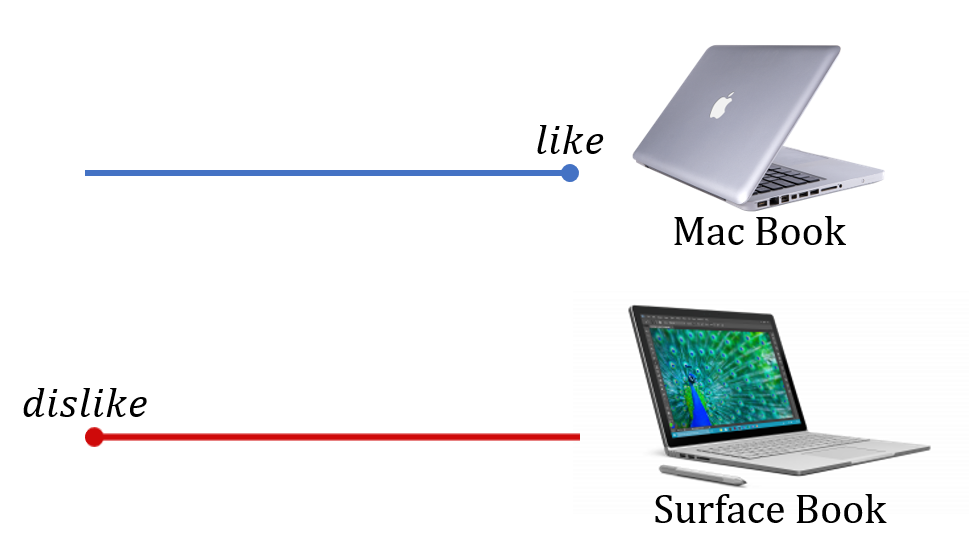
\includegraphics[width=0.45\textwidth]  {fig/single-side.png} &
			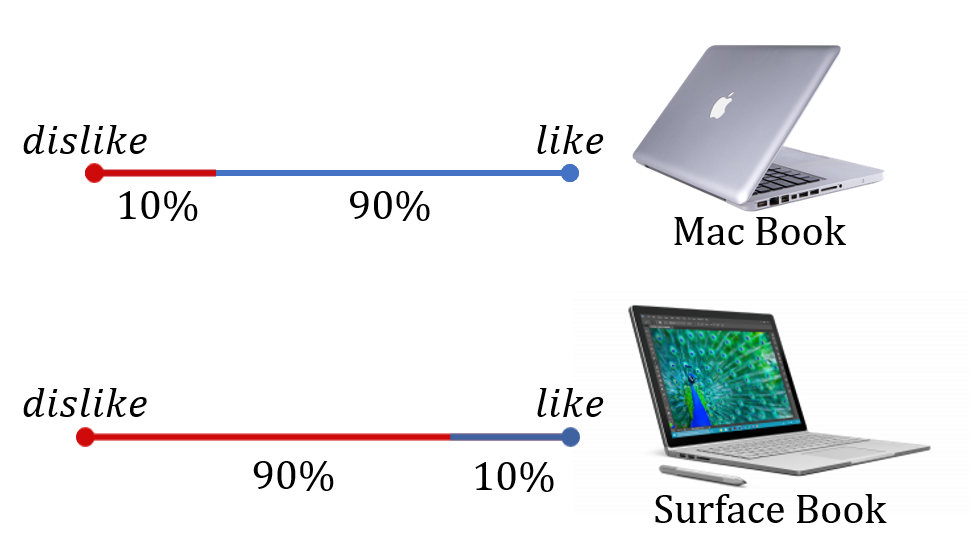
\includegraphics[width=0.45\textwidth] {fig/two-side.png} \\
			(a) Single-side Relevance & (b)Two-side Relevance
		\end{tabular}
	\end{center}
	\caption{Single-side relevance of traditional recommendation's loss (left) and two-side relevance of our ideal loss (right).}
	\label{fig:intuition}
\end{figure*}
\begin{teaserfigure}
	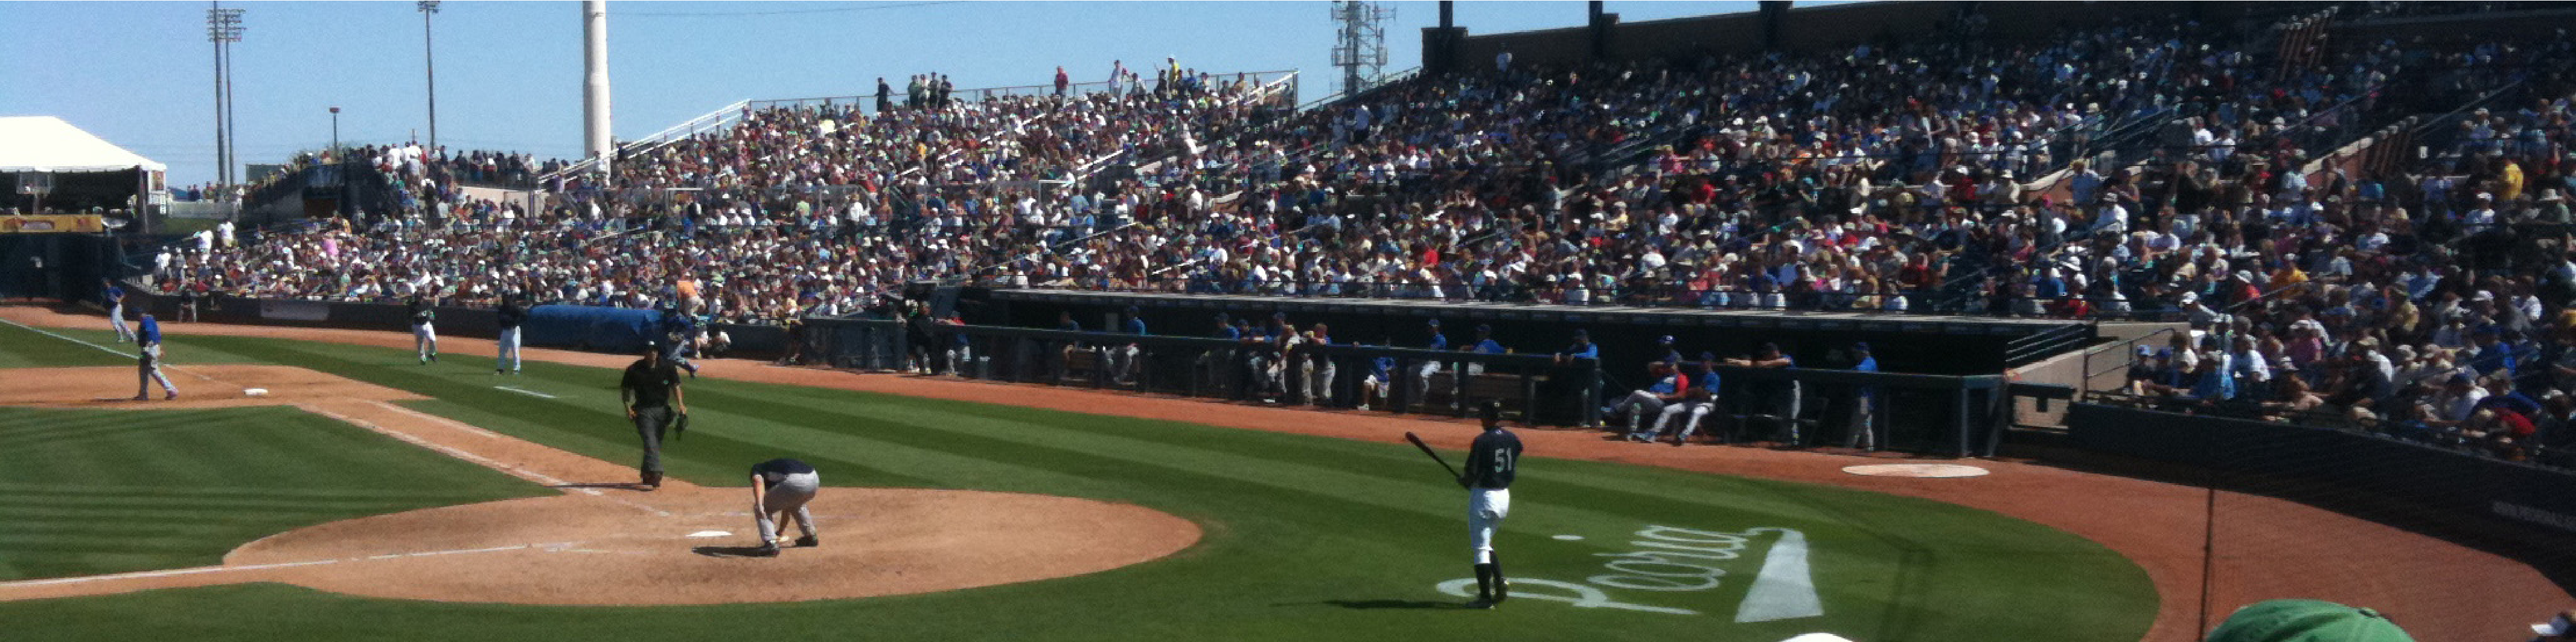
\includegraphics[width=\textwidth]{sampleteaser}
	\caption{Seattle Mariners at Spring Training, 2010.}
	\Description{Enjoying the baseball game from the third-base
		seats. Ichiro Suzuki preparing to bat.}
	\label{fig:teaser}
\end{teaserfigure}
For example, Tony is an iOS application developer and he wants to buy a new laptop. So Mac Book with iOS system is his best choice and he will click it. But sometime he needs to draw something to help others understand his application designed idea. Although Surface Book is with windows system, its screen can support for drawing. In this case, from (b) of Figure~\ref{fig:intuition}, we suppose that Tony is $90\%$ $like$ with Mac Book for its iOS system but $10\%$ $dislike$ with it for its non-drawing screen while he is $10\%$ $like$ with Surface Book for its drawing-support screen but $90\%$ $dislike$ with it for its windows system. If in traditional recommendation, Tony is supposed to be solely $100\%$ $like$ with Mac Book and $100\%$ $dislike$ with Surface Book as showed in (a) of Figure~\ref{fig:intuition}. In reality, though Tony clicks Mac Book he is not totally $like$ with it and though he does not click Surface Book he is not totally $dislike$ with it. More specially, the traditional loss function of Eq.\eqref{eq:traditionalLoss} learns based on the click data with sole and absolute $like$ or $dislike$ information (i.e. (a) of Figure~\ref{fig:intuition}) while our ideal loss function learns based on the relevance level to both $like$ and $dislike$ (i.e. (b) of Figure~\ref{fig:intuition}) , further capturing the true preferences of users. That is to say, our ideal loss models the relevance with both $like$ and $dislike$ sides (Two-side Relevance) in contrast to the traditional recommendation's single side (Single-side Relevance) with sole $like$ or $dislike$. 
\subsubsection{Transformation Function for Clipped Estimator}

Given the definition of transformation function above, we then can obtain the clipped estimator for ideal loss following Eq.\eqref{eq:clipped} as below, 
\begin{eqnarray}\label{eq:clippedTFLoss}
	\hat{\mathcal{L}}_{clipped}(\hat{R})  = \frac{1}{|\mathcal{R}|} \sum_{(u, i) \in \mathcal{R}}^{} \left[f_{c}({Y_{u,i}}, {\bar{\theta}_{u,i}}) \delta_{u, i}^{(1)} +\left(1 - f_{c}({Y_{u,i}}, {\bar{\theta}_{u,i}})\right)\delta_{u, i}^{(0)} \right] ,
\end{eqnarray}
where $f_{c}$ is the transformation function for clipped estimator (clipped function) and it can be represented as below in Eq.\eqref{eq:clipped}.
\begin{eqnarray}\label{eq:clippedTF}
	f_{c}({Y_{u,i}}, {\bar{\theta}_{u,i}}) =  \frac{Y_{u,i}}{\bar{\theta}_{u,i}}.
\end{eqnarray}

% =========================================================================================
\subsection{Na\"ive Solution with Normalization}\label{sec:navie}
% =========================================================================
Although Eq.\eqref{eq:clippedTF} can capture the relationship of Eq.\eqref{eq:cov}, it fails to capture the relevance level when $Y_{u,i} = 0$ (i.e. INCD Problem in Section~\ref{sec:rmf}). Besides it results in negative and unreasonable loss  when $Y_{u,i} = 1$ (i.e. NSL Problem in Section~\ref{sec:rmf}). As for INCD problem, we can perform a minor modification on the clipped function as below, 
\begin{eqnarray}\label{eq:clippedTFModified}
	f_{c}({Y_{u,i}}, {\bar{\theta}_{u,i}}) =  \frac{Y_{u,i} + \alpha}{\bar{\theta}_{u,i}},
\end{eqnarray}
where $\alpha$ is an adjusting variable with $\alpha = +0.01$ in negative feedback but $\alpha = -0.01$ in positive feedback. Then we further normalize the clipped function to avoid NSL problem as below,
\begin{eqnarray}\label{eq:clippedTFNormalized}
	f^{normalized}_{c}({Y_{u,i}}, {\bar{\theta}_{u,i}}) =  \frac{\frac{Y_{u,i} + \alpha}{\bar{\theta}_{u,i}}}{\max_{i' \in \mathcal{I}} \left(\frac{Y_{u,i'} + \alpha}{\bar{\theta}_{u,i'}}\right)}.
\end{eqnarray}

Although we truly avoid the above two problems and obtain better performance in experiment, we discover that there existing another problem when we visualize the normalized clipped function for user $1$ in Yahoo! R3 dataset~\footnote{http://webscope.sandbox.yahoo.com/} as Figure~\ref{fig:clickFunction}.
\begin{figure}[!htb]
	
	\begin{center}
		
		\begin{tabular}{cc}
			
			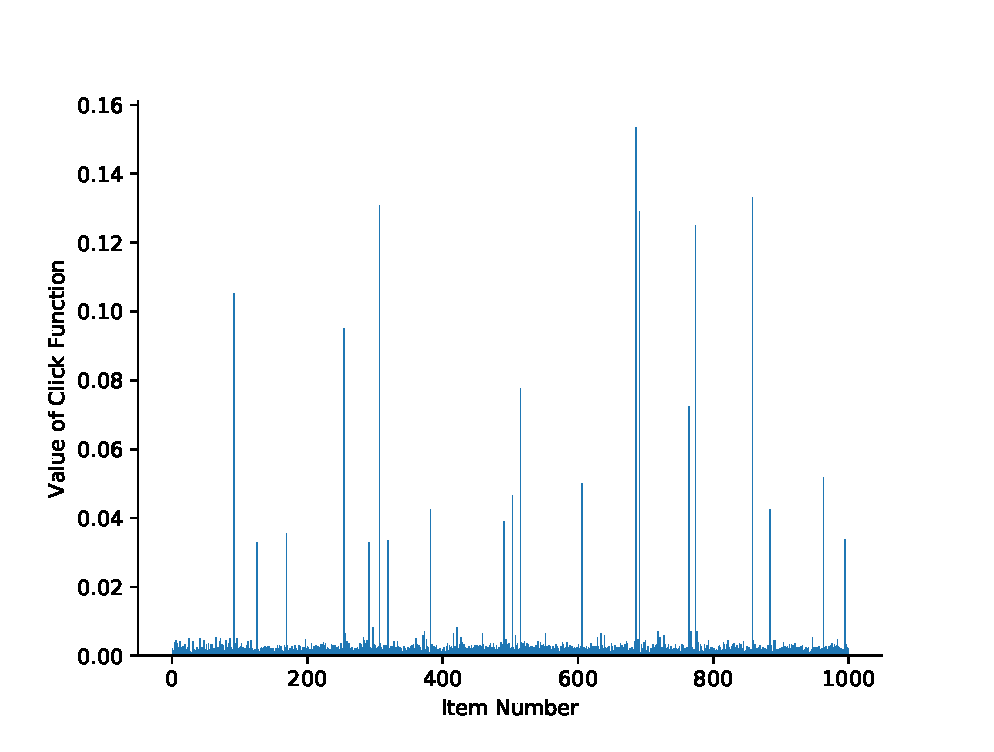
\includegraphics[width=\columnwidth]{fig/clickFunction.eps}
			
			
		\end{tabular}
		
	\end{center}
	\caption{The value of normalized clipped function for user $1$ to all items in Yahoo! R3 data.}
	
	\label{fig:clickFunction}
\end{figure} 

From Figure~\ref{fig:clickFunction} we can discover that all values of the normalized click function are even no more than 0.16, which is unreasonable because these values should be approximate to 1 which means a strong relevance in positive feedback as illustrated in Section~\ref{sec:intuition}. This problem comes from the high variance of Eq.\eqref{eq:clippedTF}, which facilitates us to design a properer clipped function.
% =========================================================================================
\subsection{Improved Solution with Power Function} \label{sec:improve}
Inspired by the intuition of Section~\ref{sec:intuition}, we design the new clipped function as below, 
\begin{eqnarray}\label{eq:clippedTFPower}
	f_{c}^{power}({Y_{u,i}}, {\bar{\theta}_{u,i}}) =  \left({Y_{u,i} + \alpha}\right)^{\bar{\theta}_{u,i}}.
\end{eqnarray}
where $\alpha = +0.01$ in negative feedback, $\alpha = -0.01$ in positive feedback. With this new clipped function we can achieve$\colon$ (\romannumeral1) the value approaches to 1 in positive feedback while the value approaches to 0 in negative feedback; (\romannumeral2) low variance in the same feedback; (\romannumeral3) keep the relationship as Eq.\eqref{eq:cov}. And we also visualize the value of this new clipped function for user $1$ in Yahoo! R3 data as Figure~\ref{fig:powerClickFunction} to help us understand the characteristics of our proposed function.

\begin{figure}[!htb]
	
	\begin{center}
		
		\begin{tabular}{cc}
			
			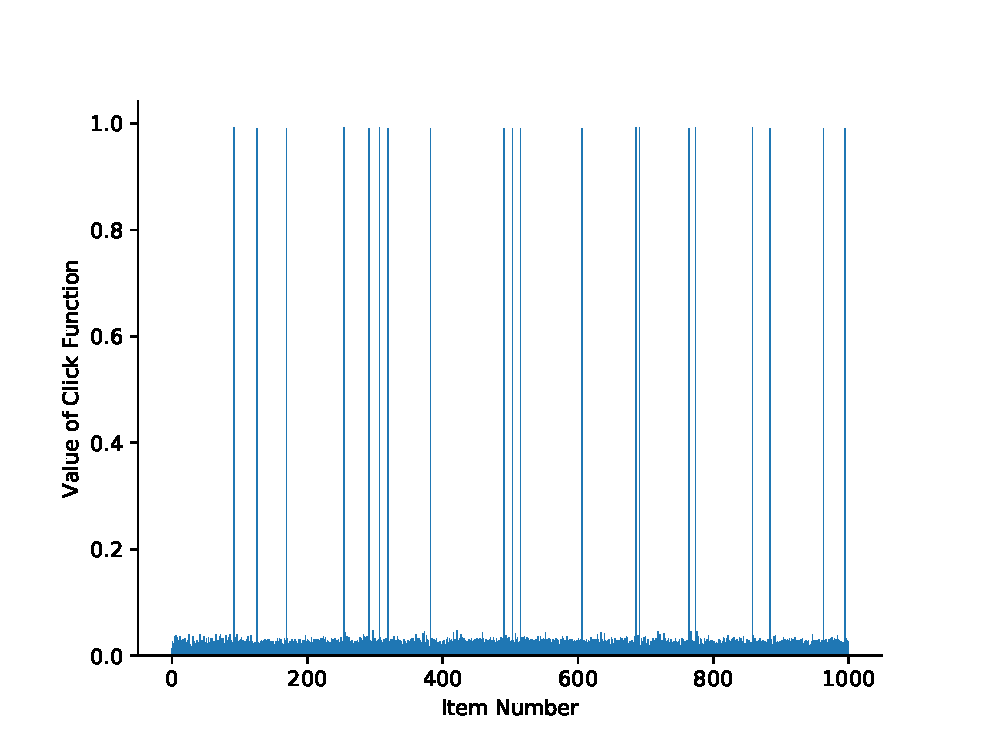
\includegraphics[width=\columnwidth]{fig/powerClickFunction.eps}
			
			
		\end{tabular}
		
	\end{center}
	\caption{The value of power clipped function for user $1$ to all items in Yahoo! R3 data.}
	
	\label{fig:powerClickFunction}
\end{figure} 

% =========================================================================================


	\subsection{Broader Perspective}
In the paper~\cite{saito2020unbiased} they only estimate the propensity score from item perspective. We further do it from user perspective and hybrid perspective as below,
\begin{eqnarray}\label{eq:useractive}
\hat{\theta}_{u,*} = \left(\frac{|\mathcal{I}_u|}{\max_{u' \in \mathcal{U}} |\mathcal{I}_{u'}|}\right)^{\eta} ,
\end{eqnarray}
%		\begin{eqnarray}\label{eq:itempop}
%	\hat{\theta}_{*,i} = \left(\frac{|\mathcal{U}_i|}{max_{i' \in \mathcal{I}} |\mathcal{U}_{i'}|}\right)^{\eta} .
%	\end{eqnarray}

\begin{eqnarray}\label{eq:hybridP}
\hat{\theta}_{u,i} = \left(\frac{|\mathcal{U}_i| \cdot |\mathcal{I}_u|} {\max_{i' \in \mathcal{I}} |\mathcal{U}_{i'}| \cdot \max_{u' \in \mathcal{U}} |\mathcal{I}_{u'}|}\right)^{\eta} ,
\end{eqnarray}
where $\eta \leq 1$. The intuition of Eq.\eqref{eq:useractive} comes from the idea that the more active users would scan the items more often and thus the items are easier to be exposed to them. Eq.\eqref{eq:hybridP} is the hybrid of Eq.\eqref{eq:itempop} and Eq.\eqref{eq:useractive}.

%	\subsection{Bucket Ranking}
%	The procedures of the bucket sort is as below.
%	\begin{enumerate}[(1)]
%		\item Normalize $\hat{r}_{ui}$ to [0, m)
%		\item Construct $m$ buckets for each user $u$
%		\item Put the item $i$ to the $\hat{r}_{ui}$th bucket of user $u$
%	\end{enumerate}
%		\begin{figure}[!htb]
%		
%		\begin{center}
%			
%			\begin{tabular}{cc}
%				
%				\includegraphics{figure=fig/bucketSort.jpg}
%				
%				
%			\end{tabular}
%			
%		\end{center}
%		\caption{Bucket Sort.}
%		
%		\label{fig:powerClickFunction}
%	\end{figure} 
%	

\subsection{Complexity}
%	\subsubsection{Complexity of Bucket Sort}
%	The space complexity and the time complexity of Bucket Sort are both $O(n \times m)$. But we can achieve no extra space cost utilizing the feedback matrix $\textbf{R}$. Because implicit feedback can be represented by digits 0 and 1, so we can store them only by one bit and utilize the left space of $\textbf{R}$ to store the item number. And the operations can be finished via binary calculation as below.
%	\begin{itemize}
%		\item Put the item $i$ to the $\hat{r}_{ui}$th bucket of user $u \colon$ $\textbf{R}_{u,\hat{r}_{ui}} = i << 1 + \textbf{R}_{u,\hat{r}_{ui}} \& 1$ 
%		\item Obtain the implicit feedback of user $u$ to item $i \colon \textbf{R}_{u,i} \& 1$
%		\item Obtain the item $i$ of user $u$ given $\hat{r}_{ui} \colon \textbf{R}_{u,\hat{r}_{ui}} >> 1$  
%	\end{itemize}
%	Besides, we also can reduce the time complexity to $O(n \times \log m)$ via divide and conquer method.
\subsubsection{Complexity of Clipped Loss}
Notice that our clipped loss learns based on the whole data with a high computational cost. The computation complexity of our clipped loss is  $O(n \times m \times d)$, but actually we can further reduce it to $O\left((n + m )\times d^2\right)$ and the proof procedures are as below,
\begin{equation}\label{eq:complexityProof}
\begin{aligned}
& \resizebox{!}{.9\height}{$\hat{\mathcal{L}}_{clipped}(\hat{R}) = \frac{1}{|\mathcal{R}|} \sum_{(u, i) \in \mathcal{R}}^{} \left[f_{c}({Y_{u,i}}, {\bar{\theta}_{u,i}}) \delta_{u, i}^{(1)} +\left(1 - f_{c}({Y_{u,i}}, {\bar{\theta}_{u,i}})\right)\delta_{u, i}^{(0)} \right] $}\\
& \resizebox{!}{.9\height}{$= \frac{1}{|\mathcal{R}|} \sum_{u \in \mathcal{U}}^{} \sum_{i \in \mathcal{I}}^{} \left[f_{c}({Y_{u,i}}, {\bar{\theta}_{u,i}}) (\hat{r}_{ui} - 1)^2 +\left(1 - f_{c}({Y_{u,i}}, {\bar{\theta}_{u,i}})\right)(\hat{r}_{ui} - 0)^2 \right]$} \\
&\resizebox{!}{.9\height}{$ = \frac{1}{|\mathcal{R}|} \sum_{u \in \mathcal{U}}^{} \sum_{i \in \mathcal{I}}^{} \left[ f_{c}({Y_{u,i}}, {\bar{\theta}_{u,i}}) (\hat{r}_{ui} - 1)^2 + {\hat{r}_{ui}}^2 - f_{c}({Y_{u,i}}, {\bar{\theta}_{u,i}}){\hat{r}_{ui}}^2  \right] $}	 \\
&\resizebox{!}{.9\height}{$= \frac{1}{|\mathcal{R}|} \sum_{u \in \mathcal{U}}^{} \sum_{i \in \mathcal{I}}^{} \left[ f_{c}({Y_{u,i}}, {\bar{\theta}_{u,i}}) (1-2{\hat{r}_{ui}}) + {\hat{r}_{ui}}^2 \right]$} \\
&\resizebox{!}{.9\height}{$= \frac{1}{|\mathcal{R}|} \sum_{u \in \mathcal{U}}^{} \sum_{i \in \mathcal{I}}^{} \left[ {\hat{r}_{ui}}^2-2f_{c}({Y_{u,i}}, {\bar{\theta}_{u,i}}) {\hat{r}_{ui}}  + f_{c}({Y_{u,i}}, {\bar{\theta}_{u,i}}) \right] $}\\ 
&\resizebox{!}{.9\height}{$= \frac{1}{|\mathcal{R}|} \sum_{u \in \mathcal{U}}^{} \sum_{i \in \mathcal{I}}^{} \left[ {\hat{r}_{ui}}^2 - 2f_{c}({Y_{u,i}}, {\bar{\theta}_{u,i}}) {\hat{r}_{ui}}  \right] + \frac{1}{|\mathcal{R}|} \sum_{u \in \mathcal{U}}^{} \sum_{i \in \mathcal{I}}^{} \left[  f_{c}({Y_{u,i}}, {\bar{\theta}_{u,i}}) \right]$} \\ 
&\resizebox{!}{.9\height}{$= \underbrace {\frac{1}{|\mathcal{R}|} \sum_{u \in \mathcal{U}}^{} \sum_{i \in \mathcal{I}}^{} \left[ {\hat{r}_{ui}}^2 - 2f_{c}({Y_{u,i}}, {\bar{\theta}_{u,i}}) {\hat{r}_{ui}}  \right]}_{(a)} + const$},
\end{aligned}
\end{equation}
where $const$ is the constant value that can be precomputed. And $(a)$ can also be further optimized following the paper~\cite{chen2019efficient} as below,
\begin{eqnarray}\label{eq:r_ui}
{\hat{r}_{ui}} = \sum_{k = 1}^{d} U_{uk} V_{ik} ,
\end{eqnarray}
\begin{eqnarray}\label{eq:r_ui^2}
{\hat{r}_{ui}}^2 = \sum_{k = 1}^{d} \sum_{l = 1}^{d} \left[ \left(U_{uk} V_{ik}\right)  \left(U_{ul} V_{il}\right) \right],
\end{eqnarray}

\begin{equation}\label{eq:complexityProofRemoveConst}
\begin{split}
 &(a) =  \\
 & \frac{1}{|\mathcal{R}|} \sum_{u \in \mathcal{U}}^{} \sum_{i \in \mathcal{I}}^{} \left[ \sum_{k = 1}^{d} \sum_{l = 1}^{d} \left[ \left(U_{uk} V_{ik}\right)  \left(U_{ul} V_{il}\right) \right] - 2f_{c}({Y_{u,i}}, {\bar{\theta}_{u,i}}) \sum_{k = 1}^{d} U_{uk} V_{ik}  \right]  \\ 
 &=  \frac{1}{|\mathcal{R}|} \sum_{k = 1}^{d} \sum_{l = 1}^{d} \left[\sum_{u \in \mathcal{U}}^{} \left(U_{uk} U_{ul}\right) \sum_{i \in \mathcal{I}}^{} \left(V_{ik} V_{il}\right)  \right] \\
 & -   \frac{2}{|\mathcal{R}|} \sum_{k = 1}^{d} \left[\sum_{u \in \mathcal{U}}^{}  U_{uk} \sum_{i \in \mathcal{I}}^{} V_{ik}  \right]
\end{split}
\end{equation} 
% =========================================================================================
\section{Experiments}
\label{sec:exp}
To illustrate the effectiveness of our improved solution with power function, we mainly focus on the following three points$\colon$ (\romannumeral1) the comparison of performance with Na\"ive Solution and Rel-MF~\cite{saito2020unbiased}; (\romannumeral2) the efficiency of the convergence and loss decrease; (\romannumeral3) the impact of different perspectives (user-perspective and hybrid-perspective). 
\subsection{Dataset and Evaluation Metrics}
We adopt Yahoo! R3 dataset following this paper~\cite{saito2020unbiased} because the item and user distributions of its training and test sets are various, as well as, its explicit feedback data makes it possible for utilizing the information of ground truth relevance in the test set. Hence, this dataset is capable for the evaluation task of recommendation with both positive-unlabeled and MNAR problems. Besides, as illustrated in this paper~\cite{yang2018unbiased}, the ratings of user towards music in this dataset are uniform-randomly selected, making it reasonable for us to model recommendation's true performance based on it.
More specially, this dataset is extracted from a song recommendation with explicit feedback, consisting of ? ratings
from ? users towards ? music. In pre-processing, we only keep the user-item pairs with ratings greater than or equal to 4 (i.e. $r_{ui} \geq 4$) as relevant, and consider all other pairs as irrelevant. 

For the clearer comparison with this paper\cite{saito2020unbiased}, we adopt $DCG@k$, $Recall@k$ and $MAP@k$ as the evaluation metrics and vary the values of $k \in \{1, 3, 5\}$ consistent with their work. 

\subsection{Baseline and Parameter setting}
In this paper~\cite{saito2020unbiased}, they propose Relevance Matrix Factorization (Rel-MF) which outperforms their two selected baselines, Weighted Matrix Factorization (WMF) ~\cite{hu2008collaborative} and Exposure Matrix Factorization (ExpoMF)~\cite{liang2016modeling} . Therefore, in this work we base on their results and only choose the best model, Rel-MF, as our baseline. If our proposed models beat Rel-MF, it is convinced that our models also can beat WMF and ExpoMF. The models of our experiments are as below.

\begin{itemize}
	\item Relevance Matrix Factorization (Rel-MF)~\cite{saito2020unbiased}$\colon$ Rel-MF is the basic recommendation model in this work. Modeling by latent features like Matrix Factorization (MF), it learns the user and item features via minimizing the loss function as Eq.\eqref{eq:clipped} and the propensity score is estimated by Eq.\eqref{eq:itempop}. 
	\item Naive Solution with Normalization for Rel-MF (NRel-MF)$\colon$ NRel-MF is our proposed model and it aims to tackle the INCD problem and NSL problem in Section~\ref{sec:rmf}. The propensity score is estimated following Rel-MF. 
	\item Improved Solution with Power Function for Rel-MF (PRel-MF)$\colon$ We further propose PRel-MF because the NRel-MF's clipped function is of high variance and we select power function which is capable for handling such problem when keeping the covariance as Eq.\eqref{eq:cov}. The propensity score is estimated by Eq.\eqref{eq:itempop} in the experiments of performance and convergence comparisons while is estimated by Eq.\eqref{eq:useractive} and Eq.\eqref{eq:hybridP} additionally in the experiment of various perspectives. 
\end{itemize}
For parameter configuration, we set the parameter for Rel-MF the same as the original paper\cite{saito2020unbiased}. For our proposed models, we fix the number of latent dimensions and regularization parameter as 200 and 0.0001, respectively, following this paper\cite{saito2020unbiased}.  We set $\eta = 0.5$ and $\eta = 0.0625$ for NRel-MF and PRel-MF, respectively. Besides, we choose the learning rate from $\{0.0005, 0.001, 0.005, 0.01\}$ and finally pick $\gamma = 0.001$ and $\gamma = 0.005$ for Rel-MF and PRel-MF, respectively. As for the iteration number, we report the ranking metrics of $T = 300$,  $T = 400$ and $T = 100$ for Rel-MF, NRel-MF and PRel-MF, respectively, in performance comparison experiment, and report the loss within 300 iterations for all models in convergence comparison experiment. In various perspectives, we set the parameters for PRel-MF following the performance comparison part.

%	In details, we compare our models with Rel-MF both in 

\subsection{Results}
\begin{figure*}[!htb]
	\begin{center}
		\begin{tabular}{ccc}
			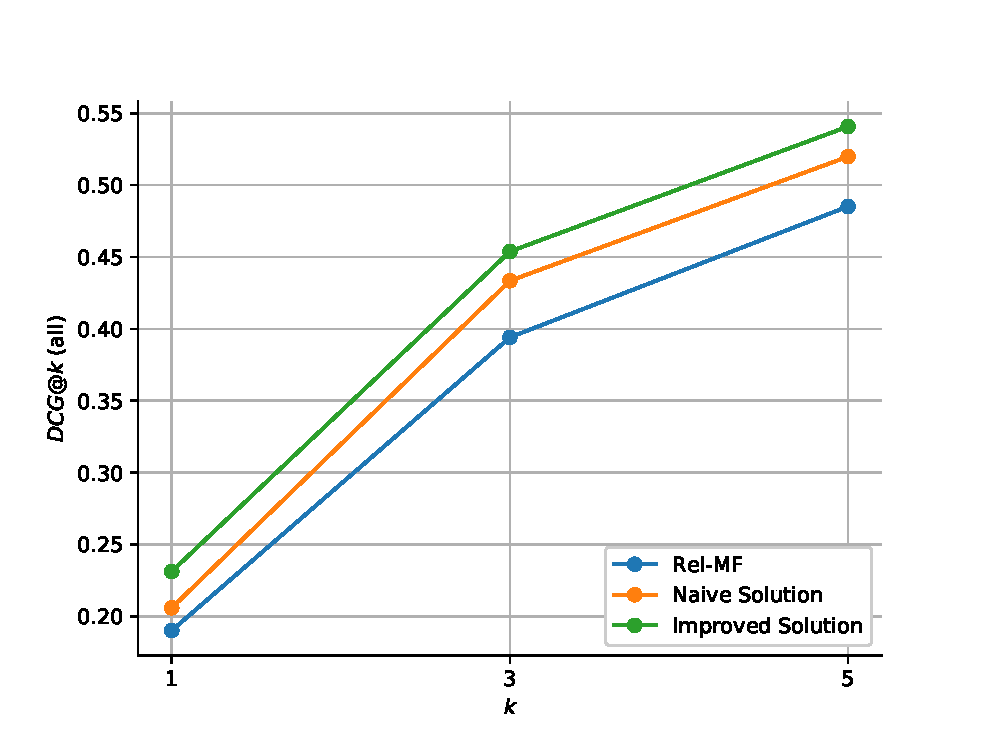
\includegraphics[width=0.3\textwidth]{fig/DCG_all.eps} &
			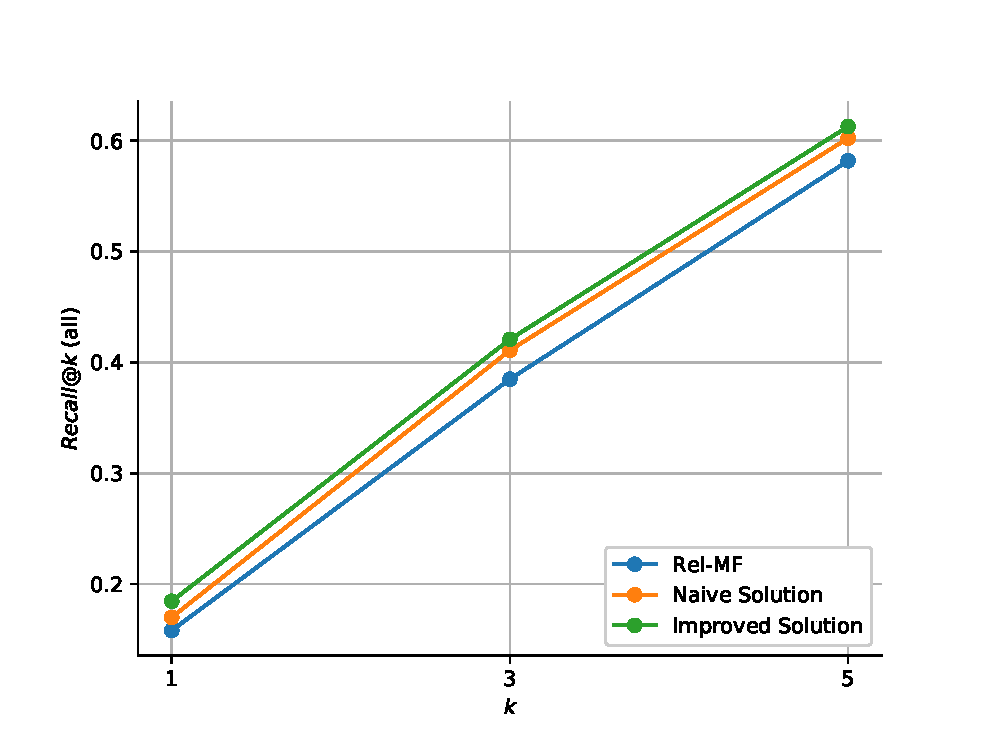
\includegraphics[width=0.3\textwidth]{fig/Recall_all.eps} & 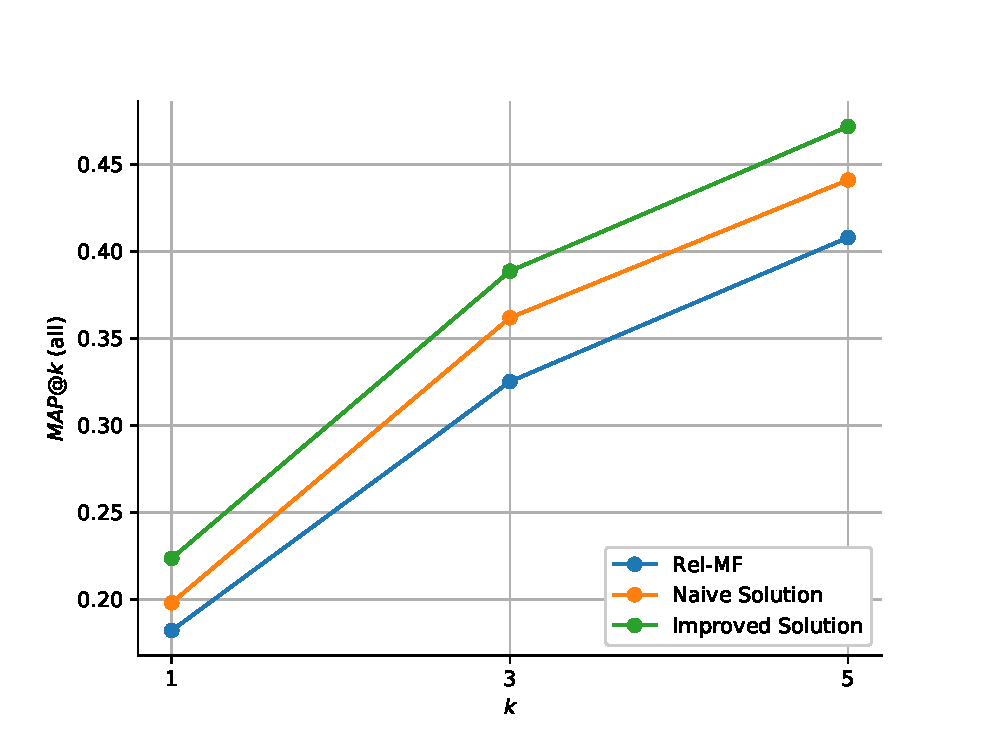
\includegraphics[width=0.3\textwidth]{fig/MAP_all.eps}	\\
			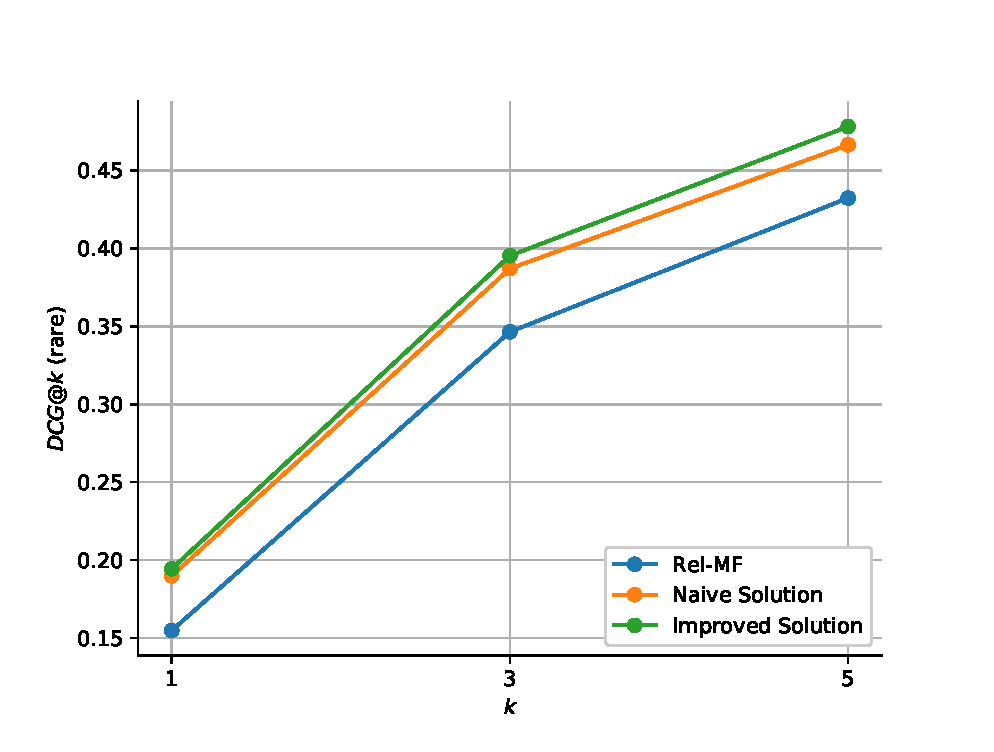
\includegraphics[width=0.3\textwidth]{fig/DCG_rare.eps} &
			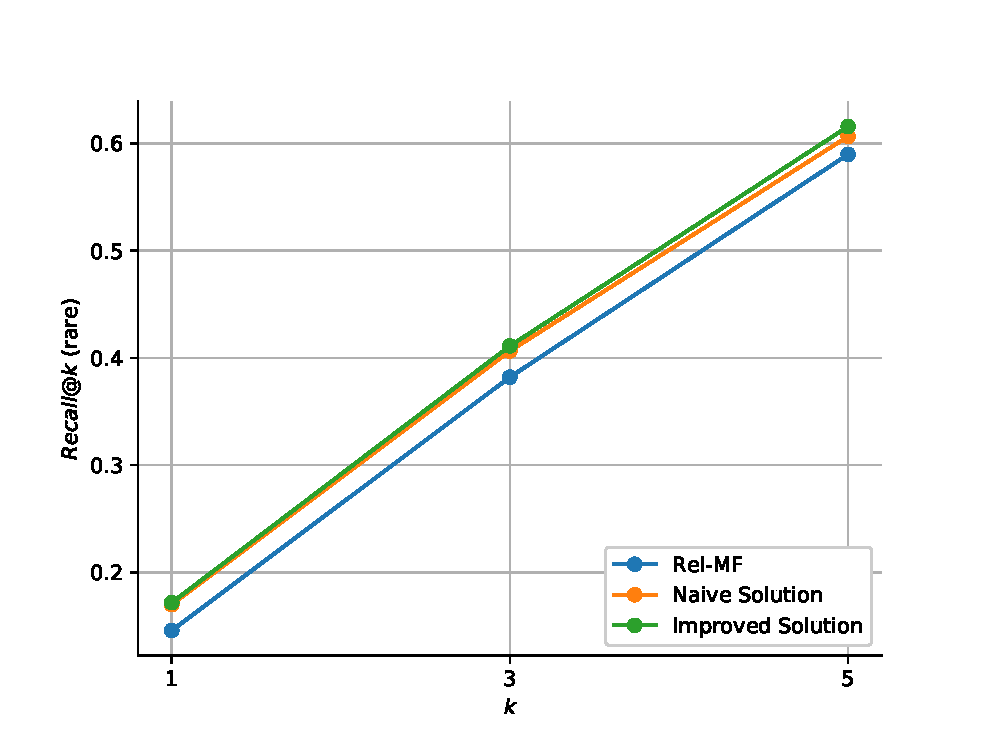
\includegraphics[width=0.3\textwidth]{fig/Recall_rare.eps} & 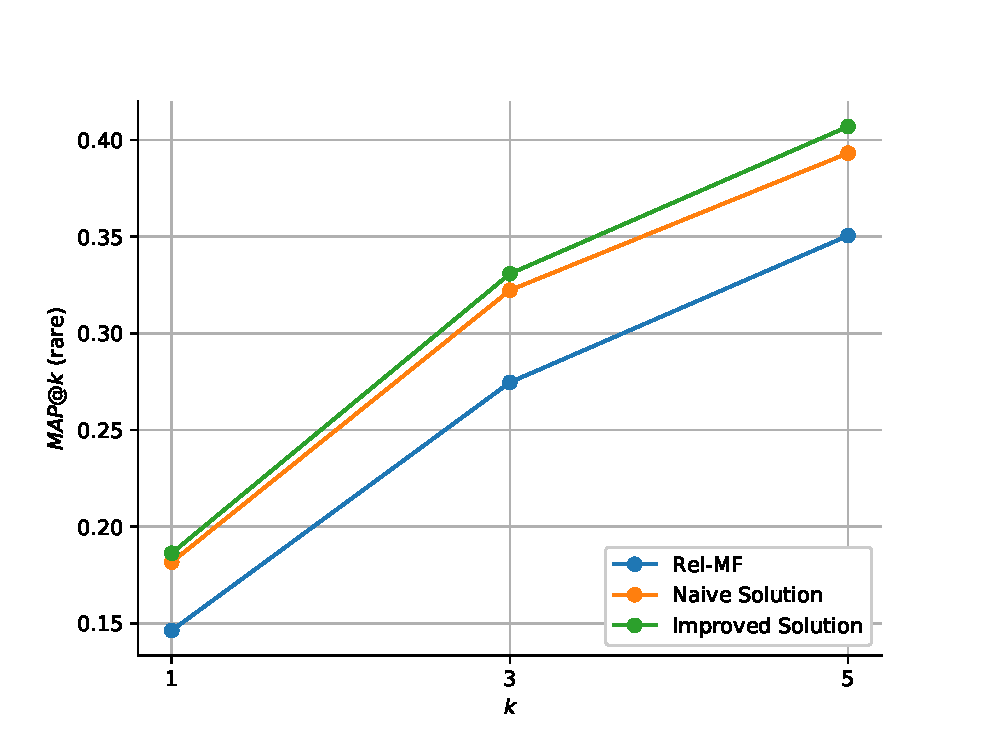
\includegraphics[width=0.3\textwidth]{fig/MAP_rare.eps}
		\end{tabular}
	\end{center}
	\caption{Ranking performance of our Improved Solution and Naive Solution against Rel-MF on the Yahoo! R3 data.}
	\label{fig:comparisonPerformance}
\end{figure*}
%\begin{figure}[ht]
%	\begin{subfigure}[width=.8\linewidth]
%		% include first image
%		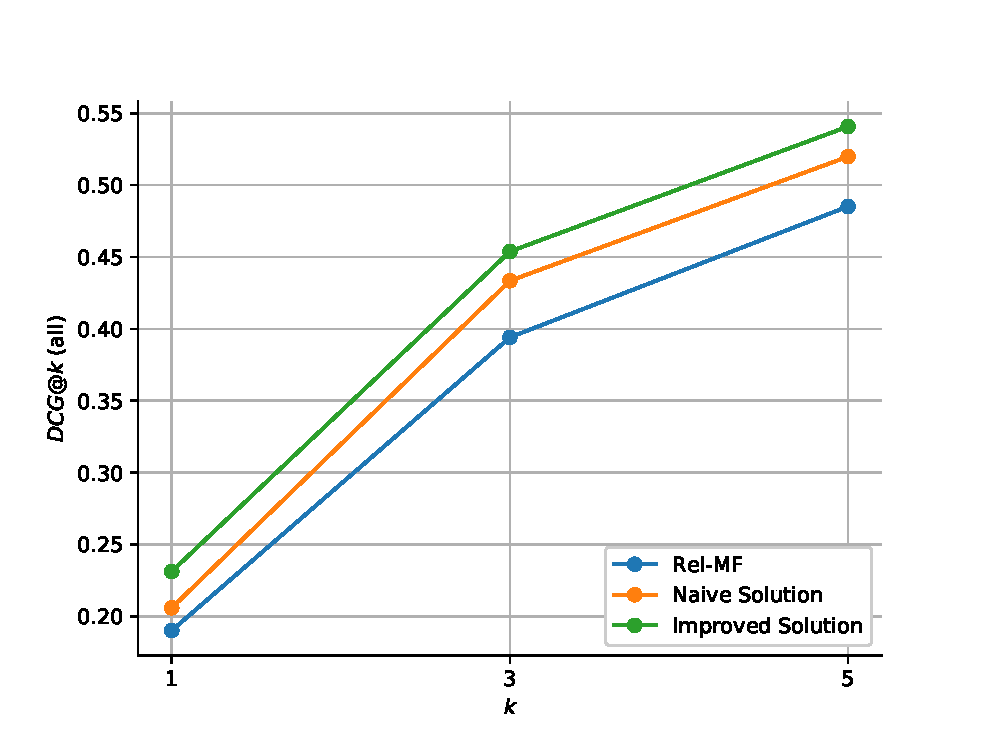
\includegraphics[width=.8\linewidth]{fig/DCG_all.eps}  
%	\end{subfigure}
%	\begin{subfigure}[width=.8\linewidth]
%		% include second image
%		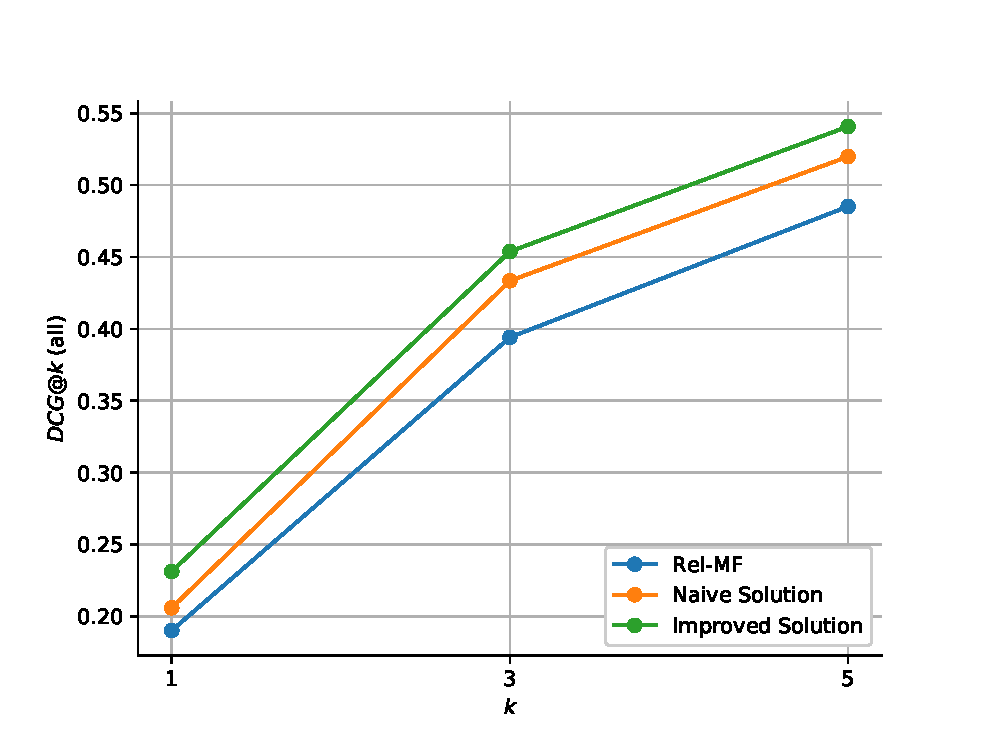
\includegraphics[width=.8\linewidth]{fig/DCG_all.eps}  
%	\end{subfigure}
%	\caption{Put your caption here}
%	\label{fig:fig}
%\end{figure}
%\begin{figure}[h!]
%	\centering
%	\begin{subfigure}[b]{.5\textwidth}
%		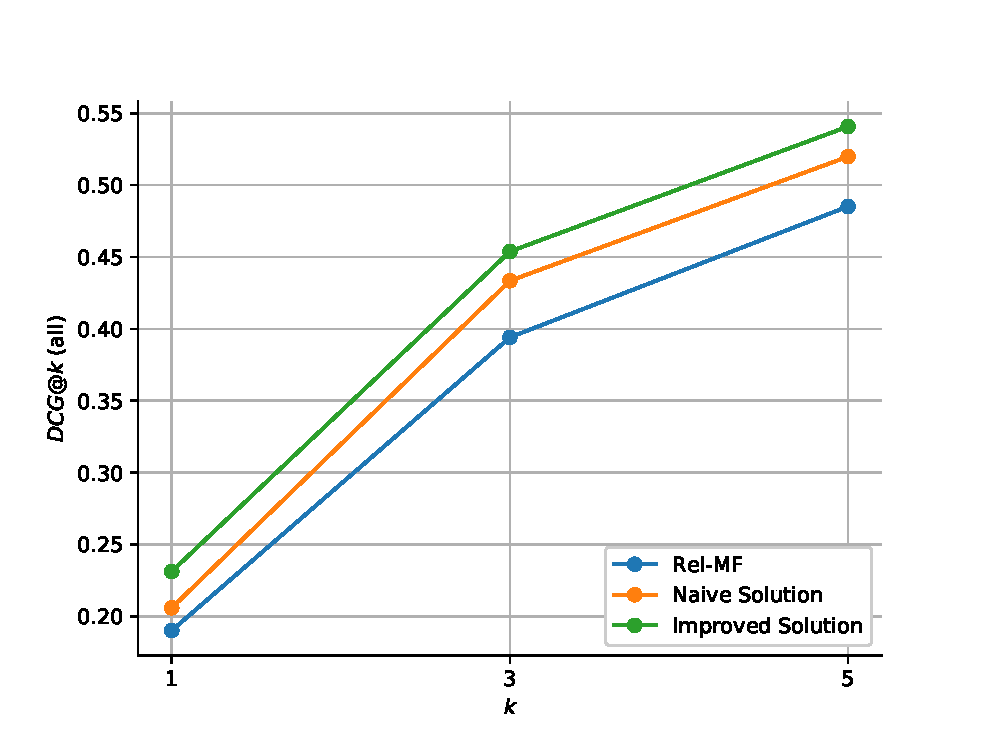
\includegraphics[width=.8\linewidth]{fig/DCG_all.eps}
%		\caption{Coffee.}
%	\end{subfigure}
%	\begin{subfigure}[b]{.5\textwidth}
%		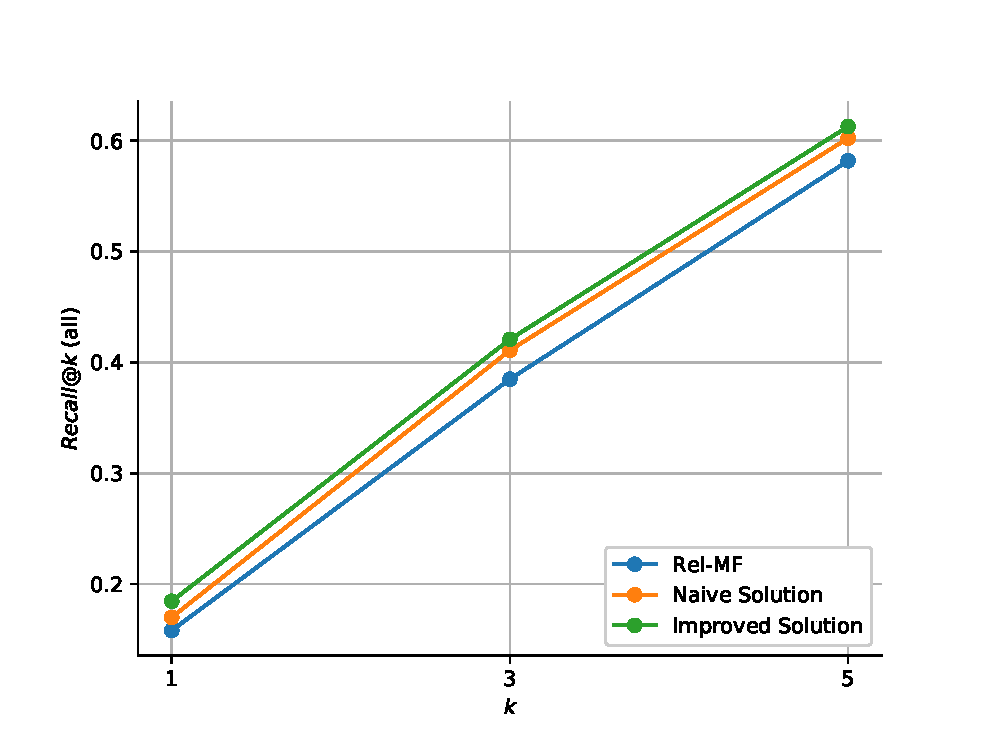
\includegraphics[width=.8\linewidth]{fig/Recall_all.eps}
%		\caption{More coffee.}
%	\end{subfigure}
%	\caption{Ranking performance of our Improved Solution and Naive Solution against Rel-MF on the Yahoo! R3 data.}
%	\label{fig:comparisonPerformance}
%\end{figure}

\paragraph{Performance Comparison}

From Figure~\ref{fig:comparisonPerformance}, we can see that both our solutions outperform Rel-MF. More specially, Naive Solution with normalization improves $DCG@5$, $Recall@5$ and $MAP@5$ by $7.15\%$, $3.50\%$ and $8.10\%$, respectively, for all items while by  $7.89\%$, $2.84\%$ and $12.16\%$, respectively, for rare items. Besides, Improved Solution with power function even further improves $DCG@5$, $Recall@5$ and $MAP@5$ by $11.46\%$, $5.31\%$ and $15.63\%$, respectively, for all items while by  $10.62\%$, $4.40\%$ and $16.10\%$, respectively, for rare items. The improvement of our Naive Solution against Rel-MF illustrates the importance of INCD problem and NSL problem we solved in Section~\ref{sec:navie}. The improvement of our Improved Solution against Rel-MF indicates the negative impact from the high variance of Eq.\eqref{eq:clippedTF} and the effectiveness of our proposed power function in Section~\ref{sec:improve}.

However, Comparing the improvements, we can easily discover that the improvements of $Recall@k$ are relatively minor, which is also similar to this paper~\cite{saito2020unbiased}. This is because the divisor of $Recall@k$ is the size of test set (i.e. $|\mathcal{I}_{u}^{te}|$) which is far greater than $k$, so the improvements of top$k$ recommendation seem relatively minor to it (i.e. $|\mathcal{I}_{u}^{te}|$).


\begin{figure}[!htb]
	\begin{center}
		
		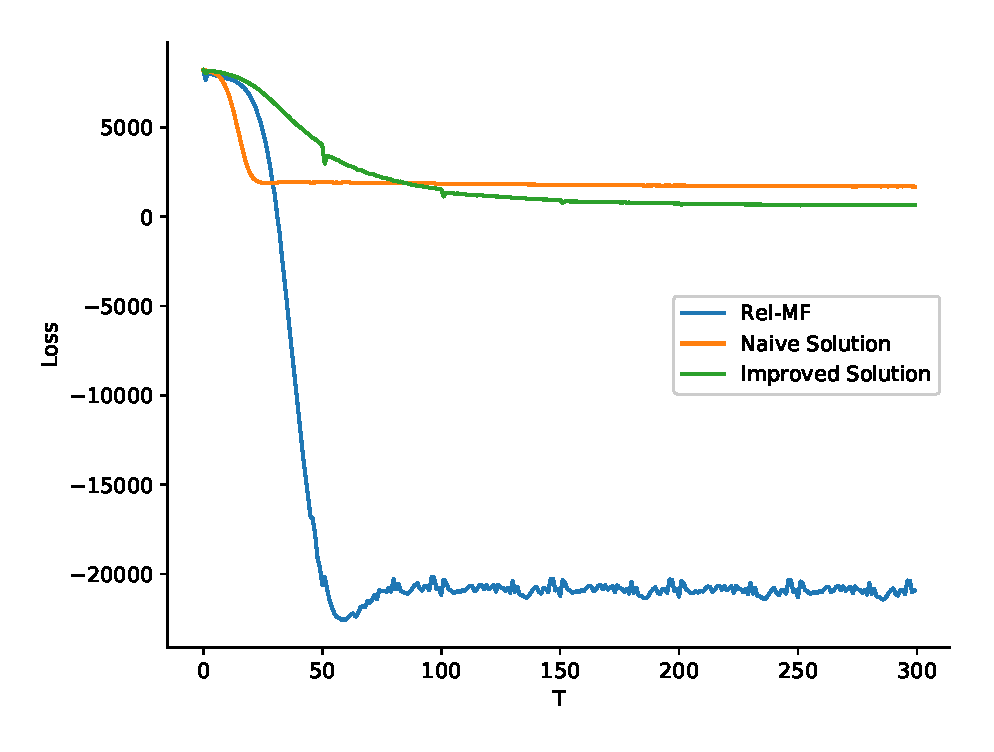
\includegraphics[width=\columnwidth]{fig/loss.eps}
		
	\end{center}
	\caption{Loss decrease of our Improved Solution, Naive Solution and Rel-MF on the Yahoo! R3 data in 300 iterations.}
	\label{fig:loss}
\end{figure}
\paragraph{Convergence Comparison} From Figure~\ref{fig:loss} we can discover the following two key points$\colon$ (\romannumeral1) The loss decrease of Rel-MF is unreasonable because it shows negative loss in square loss whose objective value is 0 and is supposed to be greater than 0, resulting from NSL problem. Moreover, its decrease is very unsteady compared with the loss decreases of our solutions. (\romannumeral2) Although the loss decrease of our Naive Solution is faster than that of our Improved Solution, Naive Solution fails to reach better convergence. Besides, its ranking metrics drop at first but reach decent performance even after 400 iterations. The second point also further shows the effectiveness of our proposed power function and the significance of tackling the high variance of Eq.\eqref{eq:clippedTF}.
% Please add the following required packages to your document preamble:
% \usepackage{multirow}
% \usepackage[table,xcdraw]{xcolor}
% If you use beamer only pass "xcolor=table" option, i.e. \documentclass[xcolor=table]{beamer}
% \usepackage[normalem]{ulem}
% \useunder{\uline}{\ul}{}
\begin{table*}[]
	\begin{tabular}{llllllllll}
		\hline
			\hline
		\multicolumn{1}{c}{}                              & \multicolumn{3}{c}{{ \textbf{ $DCG@k$}}}                            & \multicolumn{3}{c}{{\textbf{ $Recall@k$}}}                         & \multicolumn{3}{c}{{\textbf{ $MAP@k$}}}                            \\ \cline{2-10} 
		\multicolumn{1}{c}{\multirow{-2}{*}{Perspective}} & \multicolumn{1}{c}{k = 1} & \multicolumn{1}{c}{k = 3} & \multicolumn{1}{c}{k = 5} & \multicolumn{1}{c}{k = 1} & \multicolumn{1}{c}{k = 3} & \multicolumn{1}{c}{k = 5} & \multicolumn{1}{c}{k = 1} & \multicolumn{1}{c}{k = 3} & \multicolumn{1}{c}{k = 5} \\ \hline
		Item                                              & 0.2293                    & \textbf{0.4575}           & 0.5387                    & 0.1835                    & \textbf{0.4252}           & 0.6092                    & 0.2215                    & 0.3893                    & 0.4679                    \\ \hline
		User                                              & 0.2283                    & 0.4539                    & \textbf{0.5404}           & 0.1837                    & 0.4214                    & \textbf{0.6111}           & 0.2206                    & 0.3872                    & 0.4689                    \\ \hline
		Hybrid                                            & \textbf{0.2300}           & 0.4568                    & 0.5392                    & \textbf{0.1843}           & 0.4246                    & 0.6087                    & \textbf{0.2222}           & \textbf{0.3898}           & \textbf{0.4700}           \\ \hline
	\end{tabular}
	\caption{Ranking performance of item perspective, user perspective and hybrid perspective in PRel-MF.}
\label{tbl:varPerspective}
\end{table*}
\paragraph{Various Perspectives} From Table~\ref{tbl:varPerspective}, we can discover that the performance of these three perspectives are generally compatible. Item perspective mostly outperforms user perspective when the value of $k$ is relatively minor (i.e. $k \leq 3$) while user perspective outperforms item perspective when $k$ is larger (i.e. $k = 5$). Hybrid perspective is the combination of item perspective and user perspective and outperforms them in more situations.
% =========================================================================================
\section{Conclusions and Future Work}
In this paper, we establish a solider theory with relevance-capturing transformation function and include existing work (i.e. Rel-MF) in bias-aware recommendation~\cite{saito2020unbiased} to our more general loss function at first. Next, we explore the problems of Rel-MF and tackle them with NRel-MF (Naive Solution with Normalization for Rel-MF), introducing an adjusting variable and normalizing naively. Then based on the analysis we discover that there is a high variance problem of Rel-MF's propensity score estimation approach and further resolve it via a designed power function. Besides, we also consider the way to estimate the propensity score from user perspective and hybrid perspective. We are also the first one to consider the computational cost problem in bias-aware recommendation. Experimental results verify the strength of our proposed models both from performance and loss decrease even in unpopular items. Broader perspectives of propensity score's estimation shows that item perspective beats user perspective with fewer recommended items while adverse situation is seen with more recommended items and the combination of them, hybrid perspective, is properer to be more decent. 

In the future, the more close-to-reality design of transformation function will be the next main focus. As it is the significant function to capture the relationship of relevance level with the click probability and exposure probability, its improvement will lead to a less bias model. Apart from that, the estimation of propensity score is a key way to represent exposure probability, having an important impact on the transformation function. So the extension on the estimation of propensity score is also waiting for us. Besides, pair-wise recommendation with bias awareness is also another interesting field need to be explored. 
\clearpage
	\bibliographystyle{plain}
\bibliography{sample-base}
\end{document}
\endinput
%%
%% End of file `sample-sigconf.tex'.
